\documentclass{beamer}
\usepackage{amsmath}
\usepackage{rotating}
\usepackage{graphicx}
\usepackage{multimedia}

\useinnertheme[shadow=true]{rounded}
\useoutertheme{shadow}
\usecolortheme{orchid}
\usecolortheme{whale}

\mode<presentation>

\newcommand{\dif}{\, \mathrm{d}}
\newcommand{\diff}[2]{\frac{\mathrm{d}#1}{\mathrm{d}#2}}
\newcommand{\partdiff}[2]{\frac{\partial #1}{\partial #2}}


\title{TMA4280 - Introduction to supercomputing}
\subtitle{The tool - properties and flaws}
\author{Arne Morten Kvarving}
\institute{NTNU and SINTEF ICT}
\date{January 2014}

\begin{document}

\maketitle


\begin{frame}\frametitle{The tool}
  \begin{itemize}
    \item We here view the computer as a \emph{tool} - a means to reach a goal.
    \item Not a course in computer science, but a course in using this tool.
    \item No sane person would ever use the hammer without getting proper instructions!
  \end{itemize}
  \begin{center}
    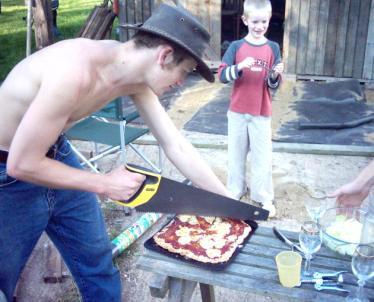
\includegraphics[width=5cm]{wrong-tool-pizza}
  \end{center}
  Image shamelessly stolen from the interwebs.
\end{frame}

\begin{frame}\frametitle{Single processor systems: RISC architecture}
Prototypical processor
\begin{center}
  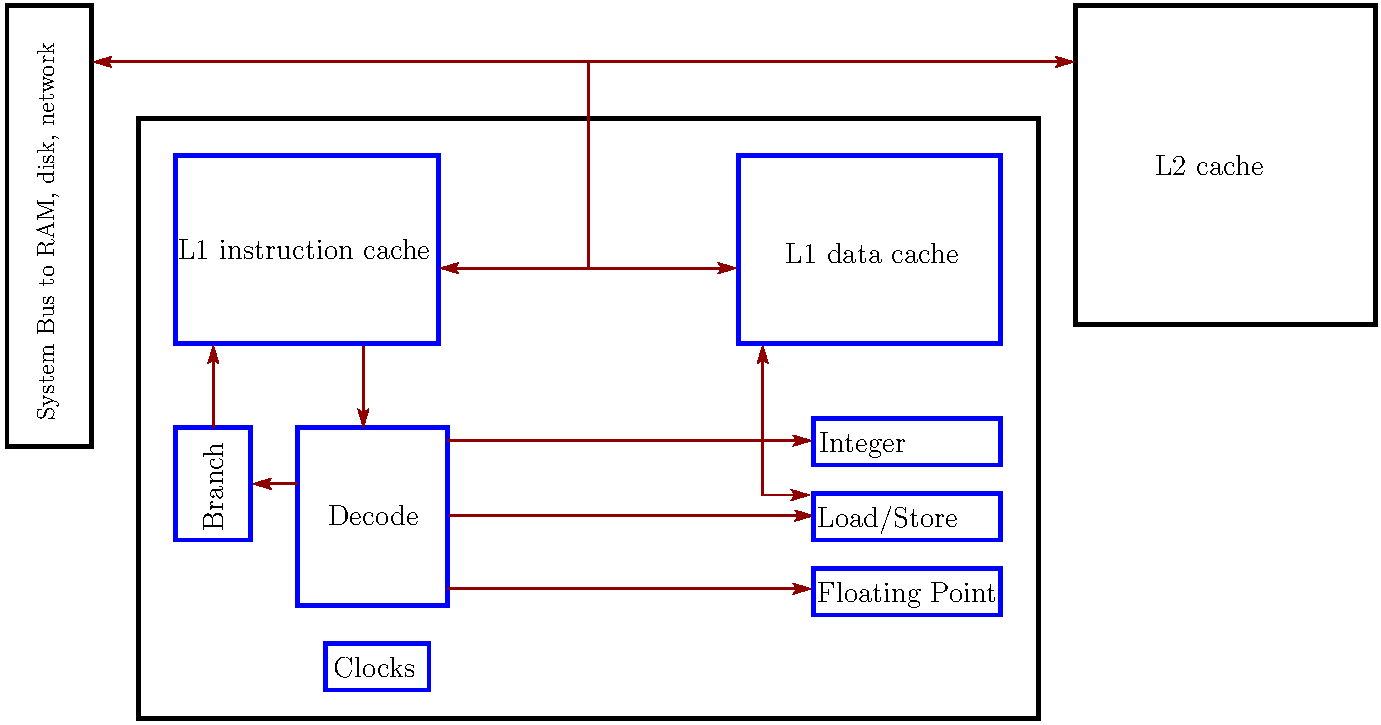
\includegraphics[width=11cm]{../../notes/01.single/Lande}
\end{center}
\end{frame}

\begin{frame}\frametitle{Single processor systems: memory hierarchy}
  \begin{center}
    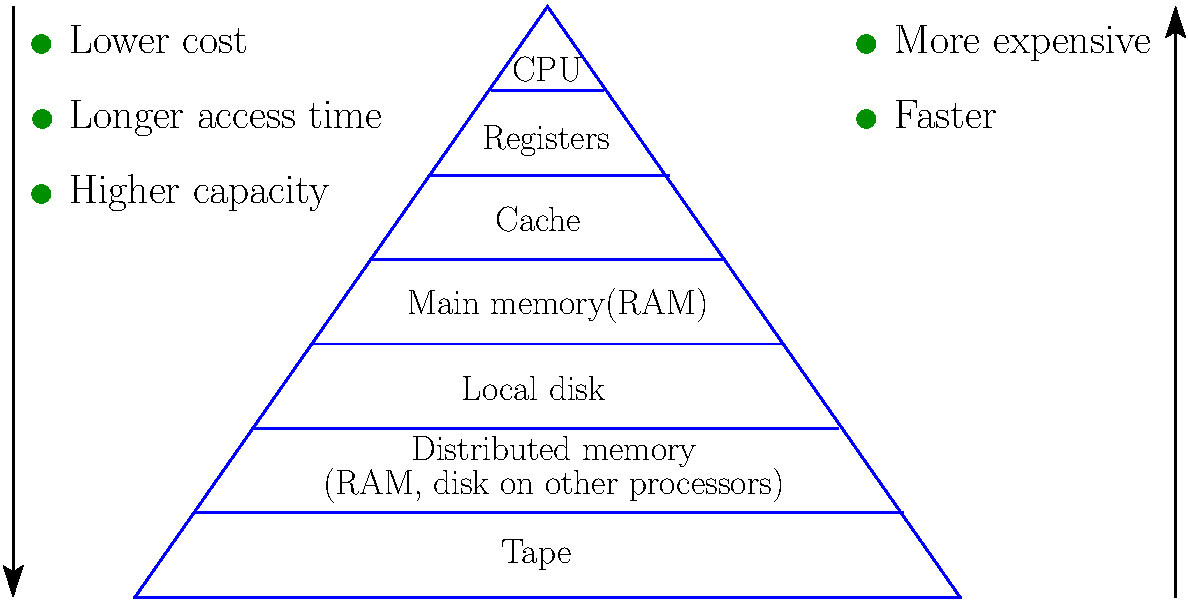
\includegraphics[width=11cm]{../../notes/01.single/MemoryHierarchy}
  \end{center}
\end{frame}

\begin{frame}\frametitle{Single processor systems: memory hierarchy}
\begin{center}
  \begin{itemize}
    \item Typical memory access times for the MIPS R14000 processor. \\
    \item The numbers represent number of clock cycles. 
    \end{itemize}
  \end{center}
  \vspace{.5cm}

  \begin{center}
    \begin{tabular}{|c|c|c|c|c|c|c|c|} \hline
      Registers & 1
        \\ \hline
      L1 cache & 2-3
        \\ \hline
      L2 cache & 10-12
        \\ \hline
      Main memory &  100-200
        \\ \hline
      Message passing & ${\cal O}(10^3)$ - ${\cal O}(10^4)$
      \\ \hline
      Local disk & ${\cal O}(10^6)$
        \\ \hline
    \end{tabular}
  \end{center}
\end{frame}

\begin{frame}\frametitle{Fixed point numbers}
  \begin{itemize}
    \item How to encode decimal numbers in the binary system?
    \item First alternative: Use x bits to represent the stuff before the comma, and
          y bits to represent the stuff after the comma, where $x+y = w$ for a $w$ bit representation.
          This is called a fixed point representation.
    \item Problem: We get a fixed range of numbers we can represent; i.e. $2^x.2^y$ is the largest.
    \item Called fixed point since the point (the comma) is fixed.
  \end{itemize}
\end{frame}

\begin{frame}\frametitle{Floating point numbers}
  \begin{itemize}
    \item A better idea is to let the comma position 'float'.
    \item Allow us to represent a much larger range of numbers.
  \end{itemize}
  \begin{figure}[htbp]
  \begin{center}
    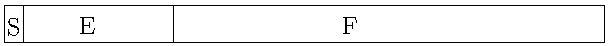
\includegraphics[scale=1]{../../notes/00.intro/ieee}
  \end{center}
  \end{figure}
  \begin{itemize}
    \item[S] The sign bit (1 bit).
    \item[E] The exponent
    \item[F] The mantissa
  \end{itemize}
\end{frame}

\begin{frame}\frametitle{Floating point numbers}
  Thus;
  \[
    N = (-1)^S 1.F \times 2^{E-B}
  \]
  for normalized representation (most common), or
  \[
    N = (-1)^S 0.F \times 2^{E-B}.
  \]
  for unnormalized numbers. Here $B$ is the \emph{bias}.
  Common precisions;
  \begin{center}
\begin{tabular}{|c|c|c|c|c|c|c|c|} \hline
Precision & $S$ & $E$ & $F$ & Total  
  \\ \hline
Single & $1$ & $8$ & $23$ & 32  
  \\ \hline
Double & $1$ & $11$ & $52$ & 64 
  \\ \hline
\end{tabular}
\end{center}
\end{frame}

\begin{frame}\frametitle{Floating point numbers}
  \begin{itemize}
    \item The \emph{bias} allows us to give a bias to large or small numbers (large or small exponents).
    \item Since we use a finite representation, we have a finite precision.
    \item Smallest number:
      \[
        V_{min} = 1\cdot 2^{1-127}\cdot 1 = 2^{-126} = 1.17\ldots 10^{-38}
      \]
      and largest number
      \[
        V_{max} = 1\cdot 2^{254-127}\cdot 2 = 3.40\ldots 10^{38}.
      \]
    \item More important: The smallest difference between numbers we can represent
      \[
        2^{-23} = 1.19....10^{-7}.
      \]
      i.e. under perfect circumstances we have about 7 digits of accuracy.
  \end{itemize}
\end{frame}

\begin{frame}\frametitle{Floating point operations}
  \begin{itemize}
    \item A very useful estimate for the size of a scientific code is the total number of floating point operations performed.
    \item Floating point operations: +, -, *, /
    \item A floating point operation is called a \emph{FLOP}.
    \item It is tempting to use FLOPs for the plural, but that is \emph{not} the norm.
    \item Rather, FLOPS is used about \emph{FLOP} per second - which is a very useful performance metric.
    \item 3 FLOP or 1 FLOP. 3 FLOPS or 1 FLOPS.
  \end{itemize}
\end{frame}

\begin{frame}\frametitle{Floating point operations - limitations}
  \begin{itemize}
    \item We have a finite precision in our number representation. This lead to some issues.
    \item Subtraction $1.2345\cdot 10^5$ minus $1.2344\cdot 10^5$.
        \[
          \begin{split}
            & 12345 - \\
            & 12344 = \\
            & 00001
          \end{split}
          \cdot 10^5
        \] 
        We have only a single digit of accuracy! This is called \emph{cancellation}.
     \item Example where this matters: Approximations of derivatives
       \[
         \frac{\mathrm{d}f}{\mathrm{d}x} \approx \frac{f(x+h)-f(x)}{h}
       \]
  \end{itemize}
\end{frame}

\begin{frame}\frametitle{Floating point operations - limitations}
  \begin{itemize}
    \item Additition: $1.2345\cdot 10^5$ plus $1.0000\cdot 10^0$.
        \[
          \begin{split}
            & 12345 + \\
            & 00001 = \\
            & 12346
          \end{split}
        \]
        OK!
      \item Additition: $1.2345\cdot 10^5$ plus $1.0000\cdot 10^{-1}$.
        \[
          \begin{split}
            & 12345 + \\
            & 00000 = \\
            & 12345
          \end{split}
        \]
        Adding the small number has no effect. This is a problem of representation accuracy only.
  \end{itemize}
\end{frame}

\begin{frame}\frametitle{Pipelining vectorization}
Consider the vector addition: 
\begin{align*}
 \underline{c} = \underline{a} + \underline{b} 
 \end{align*}
\vspace{.5cm}

We can also write this operation as the loop\\
\vspace{.5cm}
\hspace{3cm}\texttt{   for i=1,n}           \\
\hspace{4cm}\texttt{          c(i) = a(i) + b(i)}\\
\hspace{3cm}\texttt{   end} \\
Performing a flop is performed in a certain number of stages. These
stages can be viewed as a pipeline.
\end{frame}

\begin{frame}\frametitle{Superscalar operations}
\underline{a}, \underline{b}, \underline{c} are vectors\\
$\gamma$ is a scalar
\begin{align*}
 \underline{c} = \underline{a} + \gamma\, \underline{b} 
 \end{align*}
 \vspace{0.5cm}

\begin{center}
  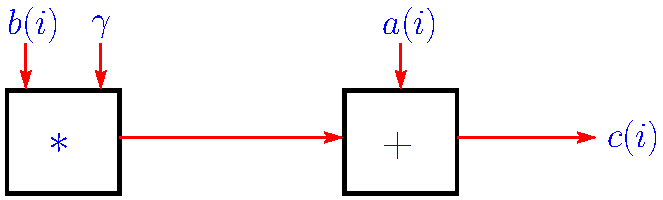
\includegraphics[width=10cm]{../../notes/01.single/SuperScalar}
\end{center}
 \vspace{0.5cm}

\begin{center}
  Fused Multiply and add (FMADD).
\end{center}
\end{frame}

\begin{frame}\frametitle{Vectorization}
Modern processors contain vector (SIMD, Single Instruction Multiple Data) units.
This allows to apply the same operation to multiple data in parallel. In
modern Intel (Sandy Bridge, Haswell) chips, the vector units are also
superscalar (both AVX and SSE).


Three ways to enable SIMD usage in your programs:
autovectorizing compilers (icc), hand-written assembly, intrinsics.
\end{frame}

\begin{frame}\frametitle{Direct mapped cache}
\begin{center}
  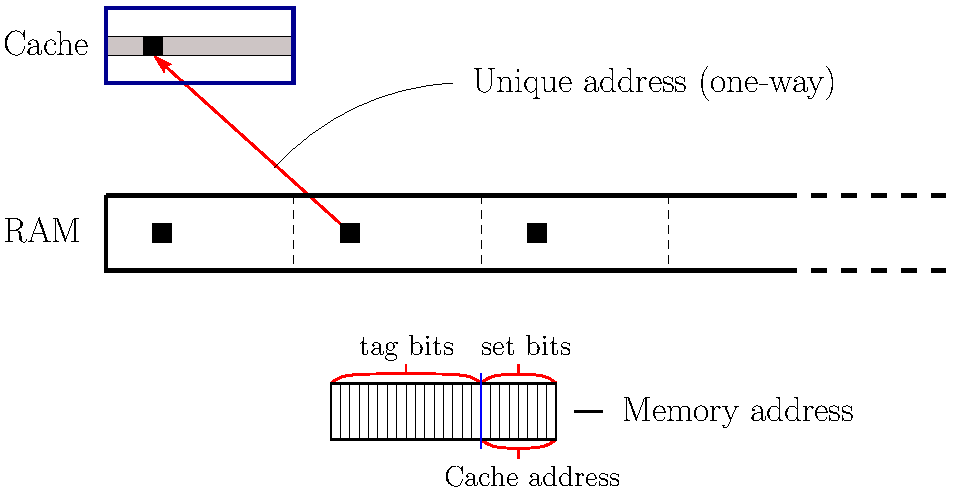
\includegraphics[width=11cm]{../../notes/01.single/DirectMappedCache}
\end{center}
\end{frame}

\begin{frame}\frametitle{Direct mapped cache: cache trashing}
\vspace{.5cm}
\hspace{3cm}\texttt{   for i=1,n}           \\
\hspace{4cm}\texttt{          c(i) = a(i) + b(i)}\\
\hspace{3cm}\texttt{   end}

\begin{center}
  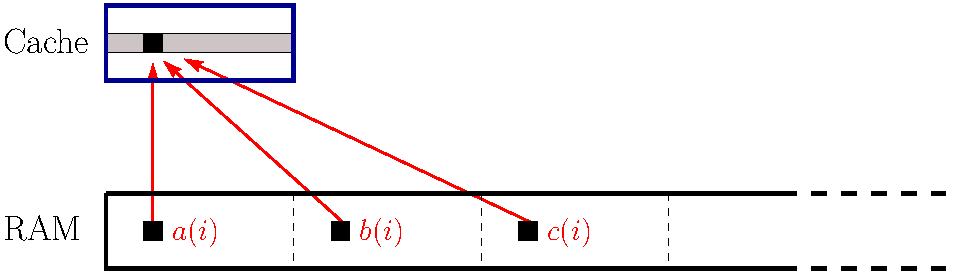
\includegraphics[width=11cm]{../../notes/01.single/CacheTrashing}
\end{center}
\end{frame}

\begin{frame}\frametitle{Direct mapped cache: avoiding cache trashing}
\begin{center}
  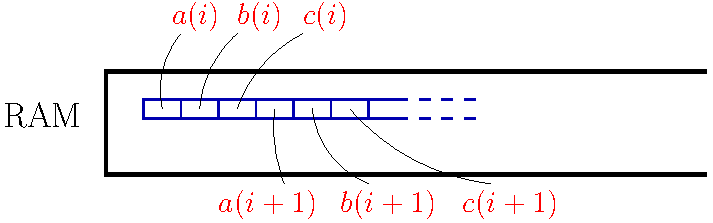
\includegraphics[width=11cm]{../../notes/01.single/AdjacentMemory}
\end{center}
\end{frame}

\begin{frame}\frametitle{n-way set-associative cache}
\begin{center}
  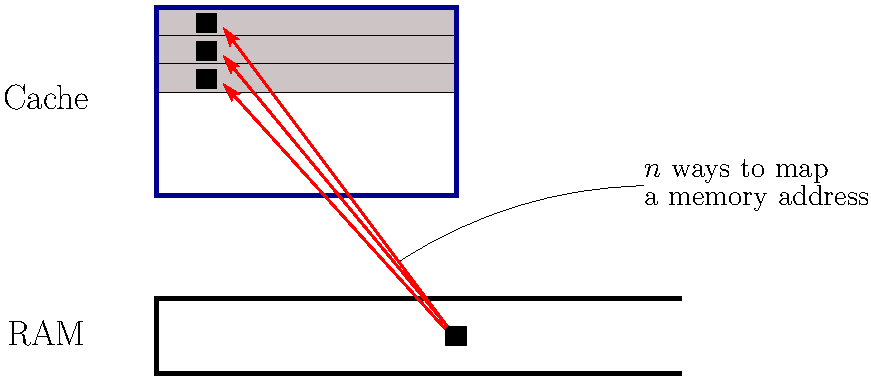
\includegraphics[width=10cm]{../../notes/01.single/NWayCache}
\end{center}
\vspace{.5cm}
Replacement policy: 
\begin{itemize}
  \item Least Recently Used (LRU)
  \item Least Frequently Used (LFU)
  \item Random
\end{itemize}
\end{frame}
\end{document}
